\documentclass[11pt,a4paper]{article}
\usepackage[margin=2.5cm]{geometry}
\usepackage{amsmath,amssymb,booktabs,tikz,listings,xcolor,enumitem}
\usepackage[colorlinks=true,linkcolor=blue!50!black]{hyperref}
\usetikzlibrary{arrows.meta,positioning}
\lstset{basicstyle=\ttfamily\small,frame=single,backgroundcolor=\color{gray!8},breaklines=true}
\title{How the rating guesser works}
\author{}
\date{}
\begin{document}
\maketitle

Codeforces gives most problems a difficulty rating, but not all of them. New problems usually have none for a while, and AtCoder and CSES use different scales altogether. This tool tries to fill that gap. If a rating exists it just shows it. If not, it guesses one from things we can measure, like how many people solved the problem, and tells you how unsure it is.

This note explains what goes in, what the models do, and where they fall short.

\section{The big picture}

Training happens once on my computer (or in GitHub Actions) and needs \texttt{numpy} and \texttt{scikit-learn}. The website itself needs nothing: the trained models are saved as plain JSON, and every guess is worked out ahead of time and stored in one file that the page just looks things up in.

\begin{center}
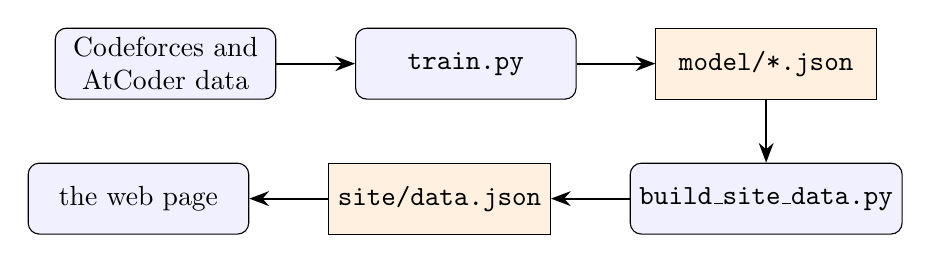
\begin{tikzpicture}[node distance=8mm and 10mm,
 b/.style={draw,rounded corners,align=center,minimum width=2.8cm,minimum height=9mm,fill=blue!6},
 s/.style={draw,align=center,minimum width=2.8cm,minimum height=9mm,fill=orange!12},
 a/.style={-{Stealth[length=2.5mm]},thick}]
\node[b](api){Codeforces and\\AtCoder data};
\node[b,right=of api](tr){\texttt{train.py}};
\node[s,right=of tr](js){\texttt{model/*.json}};
\node[b,below=of js](bd){\texttt{build\_site\_data.py}};
\node[s,left=of bd](dj){\texttt{site/data.json}};
\node[b,left=of dj](ui){the web page};
\draw[a](api)--(tr);\draw[a](tr)--(js);\draw[a](js)--(bd);\draw[a](bd)--(dj);\draw[a](dj)--(ui);
\end{tikzpicture}
\end{center}

When you paste a problem, the page decides what to show:
\begin{enumerate}[nosep]
\item Codeforces problem with a rating: show the rating.
\item Codeforces problem without one: show the model's guess and a range.
\item AtCoder task: convert AtCoder's difficulty to the Codeforces scale.
\item CSES: say there is nothing to go on.
\end{enumerate}

\section{The data}

Everything comes from public sources. From Codeforces I take every problem with its tags, its rating (if it has one) and the number of people who solved it, plus the list of contests with their names and dates. From AtCoder Problems I take the difficulty estimate for each task.

The problems that already have a Codeforces rating are my training set. The model learns what rated problems look like, then applies that to the unrated ones.

\section{What the model looks at}

Each problem becomes a list of 53 numbers. The most useful one is the number of solvers $s$, on a log scale, because hard problems get solved by fewer people. But a raw count is misleading. A Div.~3 round has far more participants than a Div.~1 round, and a problem from five years ago has had more time to collect solves. So I also give the model:

\begin{itemize}[nosep]
\item $\log\frac{s+1}{s_{\max}+1}$, the solves compared with the easiest problem in the same contest, and the problem's rank by solves;
\item the position in the contest (A, B, C, \dots) and how many problems the contest had;
\item the contest type: Div.~1, 2, 3, 4, Educational, Global or other, worked out from the contest name;
\item how old the contest is;
\item the tags, one yes/no flag per tag.
\end{itemize}

One function builds these numbers for both training and the website, so the two can't drift apart.

\section{The two models}

Let $y$ be the real rating and $\mathbf{z}$ the features after centering and scaling.

\paragraph{Ridge regression} is a straight-line fit with a penalty that keeps the weights small:
\begin{equation}
\min_{\mathbf{w},b}\ \sum_i \bigl(y_i-\mathbf{w}^{\top}\mathbf{z}_i-b\bigr)^2+\alpha\lVert\mathbf{w}\rVert^2 .
\end{equation}
The penalty matters because many features overlap (tags, contest types). I try a handful of values for $\alpha$ and keep the best.

\paragraph{Gradient boosting} builds 300 small decision trees one after another, each one fixing the mistakes of those before it:
\begin{equation}
F_m(\mathbf{x})=F_{m-1}(\mathbf{x})+\eta\,h_m(\mathbf{x}),\qquad \eta=0.05 .
\end{equation}
Trees can pick up things a straight line can't, like solve counts meaning different things in different contest types.

\paragraph{Blending.} The final guess mixes the two,
\begin{equation}
\hat y=w\,\hat y_{\text{boost}}+(1-w)\,\hat y_{\text{ridge}},
\end{equation}
with $w$ chosen from $0,0.1,\dots,1$ to give the smallest average error on held-out data. The result is rounded to the nearest 100, like real ratings.

\section{How I check it}

Problems from the same contest are similar, so if some were in the training set and others in the test set, the score would look better than it deserves. I split by contest instead (5 folds), so the model is always tested on contests it has never seen. I report the average error, the share of guesses within 100 and 200 points, and compare against the dumb baseline of always guessing the median rating. A model that can't beat that isn't worth much.

The range shown with each guess is the 10th to 90th percentile of the model's past errors, which should cover the truth about 80\% of the time. To make sure that claim holds, the training script computes the range on half the contests and counts how often it covers the other half.

\section{AtCoder}

No problem is rated on both sites, so there are no pairs to learn from. What I do instead is match percentiles. If an AtCoder problem is harder than 70\% of regular AtCoder problems, I give it the Codeforces rating that is harder than 70\% of regular Codeforces problems:
\begin{equation}
\hat r(d)=F_{\text{CF}}^{-1}\bigl(F_{\text{AT}}(d)\bigr).
\end{equation}
I do this against two sets of Codeforces problems (all regular rounds, and Div.~2/3/4 plus Educational), take the average as the guess, and use the gap between them, plus 100, as the range.

This is only a rough guide. It assumes the two communities are similarly skilled, which isn't true, and I have no way to measure how wrong it is for a single problem.

\section{Running it without scikit-learn}

Training saves the scaling numbers, the ridge weights, and every tree as lists (left child, right child, feature, threshold, value). Predicting is then plain Python:

\begin{lstlisting}[language=Python]
p=w*boost(x)+(1-w)*ridge(x)
return p,p+lo,p+hi
\end{lstlisting}

To use a tree, start at the top and go left if the feature is at most the threshold, right otherwise, until you hit a leaf.

\section{Where it falls short}

\begin{itemize}[nosep]
\item A rating reflects how real contestants performed, and solve counts only explain part of that. Expect misses of a couple of hundred points on individual problems.
\item Very new problems have few solves, so their guesses are rougher. The site says so.
\item Contests and communities change over time, so the model should be retrained now and then. GitHub Actions does that weekly.
\item The AtCoder mapping can't be validated, as explained above.
\item CSES has no data at all, so no guess.
\end{itemize}

\section{The files}

\begin{center}
\begin{tabular}{@{}ll@{}}
\toprule
\texttt{train.py} & downloads data, tests the models, saves them\\
\texttt{features.py} & turns a problem into numbers\\
\texttt{model\_runtime.py} & predicts without scikit-learn\\
\texttt{build\_site\_data.py} & works out every guess ahead of time\\
\texttt{site/} & the web page\\
\texttt{estimator.py} & live version, used by the tests\\
\texttt{app.py} & local preview server\\
\bottomrule
\end{tabular}
\end{center}

\end{document}
